% 固定来源 PDF 印刷页 86 第 23 题双曲线、渐近线及圆的结构示意重绘。
% 双曲线、圆心 A、圆半径和渐近线按题面关系作图；示意不添加未给定条件。
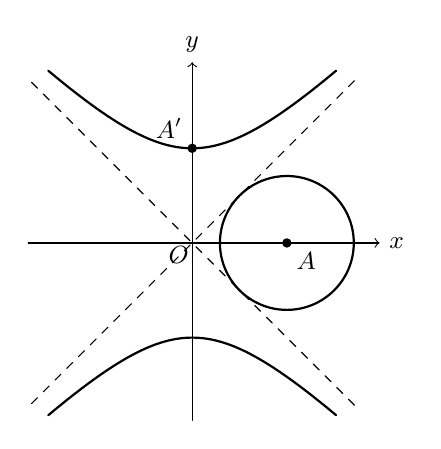
\begin{tikzpicture}[x=.85cm,y=.85cm,font=\small,line cap=round,line join=round]
  \draw[->] (-2.45,0)--(2.8,0) node[right] {$x$};
  \draw[->] (0,-2.65)--(0,2.7) node[above] {$y$};
  \draw[dashed] (-2.4,-2.4)--(2.5,2.5);
  \draw[dashed] (-2.4,2.4)--(2.5,-2.5);
  \draw[thick,domain=-2.15:2.15,samples=100,variable=\x]
    plot (\x,{sqrt(\x*\x+2)});
  \draw[thick,domain=-2.15:2.15,samples=100,variable=\x]
    plot (\x,{-sqrt(\x*\x+2)});
  \draw[thick] (1.4142,0) circle (1);
  \fill (0,1.4142) circle (1.7pt) node[above left] {$A'$};
  \fill (1.4142,0) circle (1.7pt) node[below right] {$A$};
  \node[below left,inner sep=1pt] at (0,0) {$O$};
\end{tikzpicture}
